\setcounter{chapter}{3}
\setcounter{section}{0}
\setcounter{subsection}{0}

\chapter*{Julia For Development}
The features mentioned in the previous chapter are extensively used in the 10,760 packages currently being hosted on
JuliaHub and the Julia Package Manager. The following sections will contextualize the role that Julia and its features
play in the broader field of scientific computing as well as its role in MERIT.jl. 

\section{Julia For Scientific Computing}
\label{JuliaScientificComputing}
Julia and its libraries are an attractive choice for researchers in the fields of numerical analysis, data science and
engineering. Consider the common task of solving differential equations. These equations, defined in terms of
derivatives, underpin every field of engineering from the analysis of complex electronic systems to thermodynamical
systems. The Julia package DifferentialEquations.jl \cite{rackauckas2017differentialequations} allows users to define
and solve differential equations in as little as six lines of code. Consider the example below:
\begin{lstlisting}[language=Julia]
using DifferentialEquations
f(u, p, t) = 1.01 * u
u0 = 1 / 2
tspan = (0.0, 1.0)
prob = ODEProblem(f, u0, tspan)
solution = solve(prob)
\end{lstlisting}
After defining the differential equation, initial conditions and the solution time length, the example defines an
\lstinline[language=Julia]{ODEProblem} which is a subtype of \lstinline[language=Julia]{SciMLBase.AbstractODEProblem} which
itself is subtyped from \lstinline[language=Julia]{SciMLBase.AbstractDEProblem} and this pattern continues. Notice that
the abstract type for ODEProblem was defined in the SciMLBase Module, not in the DifferentialEquations Module. SciMLBase
is a separate library that DifferentialEquations extends in a way that is completely transparent to the end user. Any
problems created using the ODEProblem type from DifferentialEquations can be used in any function from any library that
can accept the SciMLBase.AbstractODEProblem or any of its supertypes. This highlights how easy it is for new libraries
to extend older libraries in a way that is mutually beneficial for both libraries. The developer of the original library
no longer has to worry about implementing functions for every type of differential equation, and the developer of the
new library does not have to invest time in creating the complex type hierarchy or the helper functions from the
original library. Once passed to the \lstinline[language=Julia]{solve} function, the library can automatically determine
the best solver based on the problem and dispatch the relevant methods accordingly exemplifying the use of multiple
dispatch, all while boasting C and Fortran-like speeds. Their webpage demonstrates them solving the Lorenz ODE in
789.794~$\mu$s. Julia also has libraries for the field of Biology such as, but not limited to, JWAS.jl for whole genome
analysis, BioStructures.jl for manipulating macromolecules, VarientVisualization.jl for visualizing genomic variation
data and Gillespie.jl for Gillespie-type simulations in Julia. In the field of Machine Learning, there are various
libraries such as Flux.jl and TensorFlow.jl as generic machine learning libraries, BrainFlow.jl for EEG, EMG and ECG
data, and NeuralNetDiffEq.jl for physics-informed neural networks, to name a few. The easy extensibility and intuitive
interfaces that can be created using the language features in Julia make it an attractive language for developers
creating libraries and researchers who want quick answers to their questions. 

\section{Julia for MERIT.jl}
MERIT.jl also makes full use of the aforementioned features in order to create a library that is reliable, performant
and easily extensible. The sections below will outline how each feature was used to attain the goals stated at the begining.  

\subsection{Multiple Dispatch in MERIT.jl}
MERIT.jl makes use of multiple dispatch in the beamforming algorithm implementations. As mentioned before, the DAS
beamformer can be considered as a specialized case of the WDAS algorithm with a constant unit weighting factor. Due to
both being effectively the same algorithm, it was decided to combine both of these under the DAS nomenclature and use
multiple dispatch to select the correct function based on the presence of weighting factors in the argument list. This
was also used when defining the addition, subtraction and exponentiation operators so that the users can make use of the
inbuilt mathematical operators when working with the Point3 and Point2 datatypes. Multiple dispatch could also be used
in the implementation of the time domain version of the DAS beamformer, the specifics of which will be detailed in
section \ref{TDImplementation}.  

\subsection{Type Hierarchy in MERIT.jl}
The concept of abstract types and subtypes is used heavily in MERIT.jl due to the constant pace of progression in the
field. Currently, most of the research in microwave imaging is centered around breast imaging and breast cancer, however
in 2013, a pilot study published in the International Journal of Biomedical Imaging found the use of microwave imaging
to be beneficial when imaging transverse sections of the forearm \cite{gilmoreMicrowaveImagingHuman2013}. As such the
library needs to be flexible enough to adapt to novel imaging domains. The type hierarchy in MERIT.jl is centered around
the Scan abstract type, from this, the BreastScan type is subtyped which holds all the information regarding the scan
from a particular breast. In order to incorporate the aforementioned study, one would have to create a ForearmScan type,
subtyped from Scan, which has a similar field name structure to the BreastScan type. In this way, MERIT.jl achieves
extensive flexibility and expandability which would not be possible in other languages.
\begin{figure}[h!]
    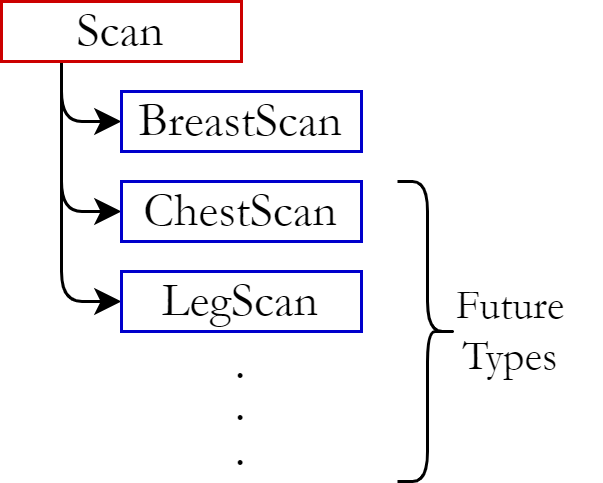
\includegraphics[width=0.5\textwidth]{scanType.png}
    \centering
    \caption{Current type hierarchy in MERIT.jl} 
    \label{fig:scanType}
\end{figure}
\FloatBarrier
This type hierarchy also synergizes with the multiple dispatch feature in Julia. Since the algorithms in MERIT.jl are
not specific to a particular body part, the one-call processing pipeline demonstrated in section \ref{CurrentWorkflow}
could easily be extended to work with any type that subtypes the Scan type, provided that the new type has a similar
field name structure to the current BreastScan struct. Full details surrounding the structure of the BreastScan struct
can be found in the Scans.jl file.

\subsection{Parametric Polymorphism in MERIT.jl}
MERIT.jl makes use of parametric polymorphism so that the functions it implements can be agnostic to the data type of
its inputs. When instantiating the BreastScan struct the user can provide the types of the data that will be loaded and
can therefore set the internal data type of the struct. It would be impossible to support all 4,176 different
permutations of every type pairing, however, with parametric polymorphism, each function only needs to be defined once
and the Julia compiler will handle the rest. This means that researchers and developers don't have to worry about
whether the library functions can support the data type of their data, so long as it follows the type restriction set on
the function, it will produce an output, creating an intuitive and easy coding experience. 

\subsection{Type Stability in MERIT.jl}
As shown in section \ref{TypeStability}, the performance gained by writing type stable code can be significant. These
gains become important when considering the many millions of function calls required to generate an output in MERIT.jl.
Consider just the distance calculations required between an $8$~cm radius breast whose domain is discretized with a
resolution of $0.25$~cm and an antenna array made of 60 antennas; this equates to roughly 4.2 million calculations alone
for each image. Performing this on a type unstable function would take far too long to compute, rendering the library
unusable. Herein lies one of the drawbacks of writing Julia code, namely, the ease at which an inexperienced developer
can write type unstable functions. In the simple case in section \ref{TypeStability}, the cause for the type instability
is evident, however, with larger more complex functions it can be hard to narrow down the cause for the instability. The
language does however, offer the \lstinline[language=Julia]{@code_warntype} macro that can analyze sections of code and
indicate, but not fix, places of instability where the compiler fails to infer the data type of the variable. This tool
can considerably benefit developers of MERIT.jl to ensure that any extensions written for the language align
with its philosophy of performance.

\subsection{Closure in MERIT.jl}
\label{ClosureMJL}
Closure, in MERIT.jl, was the programming paradigm that was used in order to achieve some customizability for the
functions that required it. Currently, it is being used in the \lstinline[language=Julia]{get_delys} in the Breamform.jl
file. Earlier sections showed how $\varepsilon$ is a free parameter in the beamforming equations, one that researchers
would be changing frequently to find the optimal parameter for each particular scan. This allows researchers to quickly
create a set of parametrized delay functions that can be easily interpolated into the BreastScan struct to be used in
the one-call processing pipeline, allowing them to answer questions regarding the optimal range for $\varepsilon$
depending on the body part or tissue composition.

\subsection{Type Safety in MERIT.jl}
The MERIT.jl library exemplifies the idea of ``strong'' type safety through its implementation of the Point data type.
The Point type is an abstract type from which the Point3 and Point2 concrete type subsets. These are lightweight
wrappers around a grouping of 3 and 2 numerical types respectively and serve the purpose of being a 3D and 2D point.
\begin{lstlisting}[language=Julia]
abstract type Point end

# xyz can be any data type that is a subset of Real
mutable struct Point3{T <: Real} <: Point
    x::T
    y::T
    z::T 
end

mutable struct Point2{T <:  Real} <: Point
    x::T
    y::T
end
\end{lstlisting}
Due to the custom nature of these data types, the inbuilt operators could not be used on them. So in addition, MERIT.jl
had to extend the in-built operators using the concepts of multiple dispatch and parametric polymorphism as mentioned
before such that these types could be useful. The full suite of implemented operators can be found in the GitHub
repository. Every function in the library that needs to work with points accepts a collection of a Points subtype
rather than a collection of numbers. This way no other collection of numbers can be erroneously passed in place of the
Points subtypes. Some edge cases still exist however, there is nothing stopping a user from incorrectly passing a
collection of points describing antenna locations to an argument which is for points from the imaging domain. Even
though this issue still exists, clear and easy to understand documentation should make this a nonissue. It should be
noted that in its current state, MERIT.jl is not completely strongly typed, this is an area of the library which can be
improved upon in the future. 
